\documentclass[a4paper,11pt]{report}

\usepackage{fontspec}
\usepackage{newunicodechar}
\usepackage{xspace}
\usepackage{multirow,array}
\usepackage{tikz}
\usepackage{soul}
\usepackage{color}
\usepackage{mathtools}
\usetikzlibrary{calc}
\usetikzlibrary{matrix}
\usetikzlibrary{positioning}
\usepackage{forest}
\usepackage{tabularx}
\usepackage{booktabs}
%\usepackage[francais]{babel}
\renewcommand{\contentsname}{Table of contents}
\usepackage[T1,OT1]{fontenc}
%\usepackage[utf8]{inputenc}

% --- font ---
% New
\usepackage{newtxtext,newtxmath}
% Libertine
%\usepackage{libertine}
%\usepackage[libertine]{newtxmath} % pdfLatex
%\usepackage{unicode-math} % new texs
%\setmathfont{texgyrepagellamath-regular.otf} % new texs

% --- packages ---
\usepackage[top=1in, bottom=1in, left=1in, right=1in]{geometry}
\usepackage{amsopn,amssymb,amsmath}
\usepackage{listings} % source codes
\usepackage{graphicx}
\usepackage{blindtext}
\usepackage{enumitem}
\usepackage{mathtools}
\usepackage{xcolor}
\usepackage[colorlinks=false,hidelinks]{hyperref}
\usepackage{needspace}
\usepackage{pdfpages}
\usepackage{cancel}
\usepackage{pdflscape}
\usepackage{adjustbox}
\usepackage{verbatim}
\usepackage{amsmath}
\usepackage{caption}

% --- custom ---
\newcommand{\lang}[1]{\emph{#1}}
\newcommand{\er}{\textsuperscript{er} }
\newcommand{\e}{\textsuperscript{e} }
%\newcommand{\solver}{\lang{solver}}
\newcommand{\solver}{solveur}
\newcommand{\tored}[1]{{\color{red}#1}}
\newcommand{\toblue}[1]{{\color{blue}#1}}
\newcommand{\ra}[1]{\renewcommand{\arraystretch}{#1}}

\DeclareRobustCommand{\hlred}[1]{{\sethlcolor{red}\hl{#1}}}
\DeclareRobustCommand{\hlgreen}[1]{{\sethlcolor{green}\hl{#1}}}
\newcommand{\mathcolorbox}[2]{\colorbox{#1}{$#2$}}

% Constantes
\newcommand{\cst}[2][]{\ensuremath{{\color{magenta}#2} #1}\xspace}
\newcommand{\PachatcV}{\cst[\real]{\mathit{Pachat}_{ac}}}
\newcommand{\Pachatc}{\cst{\mathit{Pachat}_{ac}}}
\newcommand{\PventeacV}{\cst[\real]{\mathit{Pvente}_{ac}}}
\newcommand{\Pventeac}{\cst{\mathit{Pvente}_{ac}}}
\newcommand{\PventeamcV}{\cst[\real]{\mathit{Pvente}_{(a-1)c}}}
\newcommand{\Pventeamc}{\cst{\mathit{Pvente}_{(a-1)c}}}
\newcommand{\diV}{\cst[\real]{d_i}}
\newcommand{\di}{\cst{d_i}}
\newcommand{\eijvV}{\cst[\bin]{e_{ijv}}}
\newcommand{\eijv}{\cst{e_{ijv}}}
\newcommand{\kapvV}{\cst[\naturel]{k_{apv}}}
\newcommand{\kapv}{\cst{k_{apv}}}
\newcommand{\nprimeacV}{\cst[\bin]{n'_{(a-1)c}}}
\newcommand{\nprimeac}{\cst{n'_{(a-1)c}}}
\newcommand{\ucV}{\cst[\bin]{u_c}}
\newcommand{\uc}{\cst{u_c}}

% Variables de décision
\newcommand{\var}[2][]{\ensuremath{{\color{blue}#2} #1}\xspace}
\newcommand{\gac}{\var{g_{ac}}}
\newcommand{\gacV}{\var[\bin]{g_{ac}}}
\newcommand{\hac}{\var{h_{ac}}}
\newcommand{\hacV}{\var[\bin]{h_{ac}}}
\newcommand{\nac}{\var{n_{ac}}}
\newcommand{\nacV}{\var[\bin]{n_{ac}}}
\newcommand{\qacjpv}{\var{q_{acijpv}}}
\newcommand{\qacjpvV}{\var[\real]{q_{acijpv}}}
\newcommand{\wac}{\var{w_{ac}}}
\newcommand{\wacV}{\var[\bin]{w_{ac}}}
\newcommand{\xaci}{\var{x_{aci}}}
\newcommand{\xaciV}{\var[\in \{0,\dots,251\}]{x_{aci}}}

% Variables de linéarisation
\newcommand{\varl}[2][]{\ensuremath{{\color{brown}#2} #1}\xspace}
\newcommand{\lac}{\varl{l_{ac}}}
\newcommand{\lacV}{\varl[\real]{l_{ac}}}
\newcommand{\racjpv}{\varl{r_{acijpv}}}
\newcommand{\racjpvV}{\varl[\real]{r_{acijpv}}}
\newcommand{\zacp}{\varl{z_{acp}}}
\newcommand{\zacpV}{\varl[\bin]{z_{acp}}}

% Pour tout
\newcommand{\forallin}[2]{\ \forall #1 \in #2}
\newcommand{\foralla}{\forallin{a}{A}}
\newcommand{\forallc}{\forallin{c}{C}}
\newcommand{\foralli}{\forallin{i}{I}}
\newcommand{\forallj}{\forallin{j}{J}}
\newcommand{\foralll}{\forallin{l}{L}}
\newcommand{\forallp}{\forallin{p}{P}}
\newcommand{\forallu}{\forallin{u}{U}}
\newcommand{\forallv}{\forallin{v}{V}}

% Dans
\newcommand{\bin}{\in\{0,1\}}
\newcommand{\real}{\in \mathbb{R}^+}
\newcommand{\naturel}{\in \mathbb{N}^+}

% Textes in math mode
\newcommand{\pour}{\text{pour }}
\newcommand{\et}{\text{ et }}

\DeclareMathOperator{\xor}{XOR}

% --- sectionning ---
\makeatletter
\renewcommand\@chapapp{Partie}
\renewcommand\chapter{\par\needspace{300\p@}
                    %\if@openright\cleardoublepage\else\clearpage\fi
                    \thispagestyle{plain}%
                    \global\@topnum\z@
                    \@afterindentfalse
                    \secdef\@chapter\@schapter}
\def\@chapter[#1]#2{\ifnum \c@secnumdepth >\m@ne
                         \refstepcounter{chapter}%
                         \typeout{\@chapapp\space\thechapter.}%
                         \addcontentsline{toc}{chapter}%
                                   {\protect\numberline{\thechapter}#1}%
                    \else
                      \addcontentsline{toc}{chapter}{#1}%
                    \fi
                    \chaptermark{#1}%
                    \addtocontents{lof}{\protect\addvspace{10\p@}}%
                    \addtocontents{lot}{\protect\addvspace{10\p@}}%
                    \if@twocolumn
                      \@topnewpage[\@makechapterhead{#2}]%
                    \else
                      \@makechapterhead{#2}%
                      \@afterheading
                      \vskip 10\p@%TODO: maybe better in \@afterheading
                    \fi}
\def\@makechapterhead#1{%
  \vspace*{30\p@}%
  {\parindent \z@ \raggedright \normalfont
    \ifnum \c@secnumdepth >\m@ne
        \LARGE\bfseries\thechapter\quad
        %\vskip 20\p@
    \fi
    \interlinepenalty\@M
    \huge \bfseries #1
    %\vskip 40\p@
  }}
\makeatother
\setcounter{tocdepth}{2}

% TMP ------------------

\usepackage{easy-todo}
\usepackage{lipsum}
\makeatletter
\renewcommand{\todoii}[2]{
\ifthenelse {\equal {\@todoobeyfinal }{true}}{\ifoptionfinal {\todoenable {false}}{\todoenable {true}}}{}%
\ifthenelse {\equal {\@todoenable }{true}}{%
	\refstepcounter{todos}\noindent{\todocolor{{To do \thetodos{}. #1}}}%
	\addcontentsline {lod}{todos}{\protect {\thetodos . }#2}}{}}%
\makeatother

% --- meta data ---s
\title{INFO-F-424 Combinatorial Optimization}
\author{
	Antoine Passemiers\\
	Cédric Simar
}

% --- spec chars ---
\newunicodechar{’}{'}
%\newcommand{\bdot}{%
%	\catcode`. = 13
%	\def.{\ifmmode\mathbin{\cdot}\else\char"002E\fi}
%}
%\newcommand{\edot}{%
%	catcode`. = 12
%}


\begin{document}

\begin{titlepage}
	\centering
	{\scshape\LARGE Université Libre de Bruxelles\par}
	\vfill
	{\LARGE\bfseries INFO-F-424 Combinatorial Optimization\par
		\vspace{3ex}}
	{\itshape\Large The p-Center Problem\ \ \#1\par}
	\vfill
	\makeatletter
	{\large \@author\par}
	\vfill
	\@date\par
	\makeatother
\end{titlepage}

\tableofcontents
\newpage
\setlength\parskip{0.5ex plus1ex minus.5ex}

\chapter{Introduction}
For this project, we chose to implement the problem described in the statement entitled ``The \textit{p}-Center Problem \#1'', i.e. the vertex restricted \textit{p}-center problem, an optimization problem that requires the location of \textit{p} centers on the vertices of a given network and the allocation of the nodes to the selected centers in order to minimize the distance between the nodes and their assigned centers. In the case of tree networks, low order polynomial time algorithms exist to solve the \textit{p}-center problem. However, for general networks, the problem is NP-hard.\\

The formal definition of the problem is provided in the project statement as follows: ``Let $G = \left( N, E\right)$ be a given network with vertex set $N = \lbrace 1, ..., n\rbrace$ and edge set $E$. Define $d_{ij}$ as the length of a shortest path from vertex $i \in N$ to vertex $j \in N$ in the given network and $f\left(X\right) = \max_{i \in N} \min_{x \in X} d_{xi}$ for any point set $X \subset G$. Then, the vertex restricted \textit{p}-center problem is to find a set $X^{*} \subseteq N$ with $|X^{*}| = p$ so that $f\left(X^{*}\right) \leq f\left(X\right)$ for any $X \subseteq N$ with $|X| = p$''.\\

In order to solve the vertex restricted \textit{p}-center problem, this work implements two integer programming (IP) formulations, i.e. a first formulation (P1) proposed by Daskin (1995) and a second formulation (P3) proposed by Calik and Tansel (2013).\\

In this report, we will first describe both P1 and P3 mathematical formulations, our computational experiments as well as discuss the results obtained using two different solvers interfaced by the JuMP modeling language.

\newpage
\chapter{Mathematical Formulations}
\section{P1}
The P1 formulation to solve the vertex restricted \textit{p}-center problem was proposed by Daskin (1995).
\subsection{Constants}
Let:
\begin{itemize}
	\item $G = \left( N, E\right)$ be a given network
	\item $N = \lbrace 1, ..., n\rbrace$ be the vertex set of $G$
	\item $E$ be the edge set of $G$ (not used in the vertex restricted \textit{p}-center problem)
	\item $d_{ij} \in \mathbb{N}^+$ be the length of a shortest path in $G$ from vertex $i \in N$ to vertex $j \in N$
	\item $p \in \mathbb{N}^+$ be the maximum number of centers
\end{itemize}
\subsection{Variables}
Let:
\begin{itemize}
	\item $x_{ij} \in \lbrace 0, 1\rbrace$ be $1$ if vertex $i$ assigns to a center placed at vertex $j$, $0$ otherwise
	\item $y_{j} \in \lbrace 0, 1\rbrace$ be $1$ if a center is placed at vertex $j$, $0$ otherwise
\end{itemize}
\subsection{Objective function and constraints}
The objective is to minimize\\ $$z$$\\ with respect to the variables $x_{ij}$ and $y_{j}$ under the following constraints:\\

\renewcommand{\arraystretch}{2}
\begin{tabularx}{\textwidth}{l l X r}
$\sum\limits_{j \in N} d_{ij} x_{ij}\leq z$ & $\forall i \in N$ & ensures that the objective value is no less than the maximum vertex-to-center distance & (1)\\
$\sum\limits_{j \in N} x_{ij} = 1$ & $\forall i \in N$ & assigns each vertex to exactly one center & (2)\\
$x_{ij} \leq y_j$ & $\forall i, j \in N$ & ensures that no vertex assigns to vertex $j$ unless there is a center \ \ \ \ \ \ \ \ \ \ \ \ \ \ \ at vertex $j$ & (3)\\
$\sum\limits_{j \in N} y_{j} \leq p$ & & restricts the number of centers to at most p & (4)\\
$y_{j} \in \lbrace 0, 1\rbrace$ & $\forall j \in N$ & binary restriction & (5)\\
$x_{ij} \in \lbrace 0, 1\rbrace$ & $\forall i, j \in N$ & binary restriction  & (6)
\end{tabularx}

\section{P3}
The P3 formulation to solve the \textit{p}-center problem was proposed by Calik and Tansel (2013). P3 is based on a previous Integer Programming formulation (P2) by Elloumi et al. (2004). We note that P3 extends P1 formulation to \textit{p}-FC, i.e. the F-restricted \textit{p}-center problem with $F$ being any finite subset of $G$,  by replacing ``$j \in N$'' by ``$j \in M$''. P3 used a set-covering based approach that takes advantage of the fact that the distances $d_{ij}$ are the only possible values for $r_p(F)$, i.e. the optimal p-radii of the F-restricted p-centers. This approach led to reduce the number of constraints from 6 (P1) to 5 (P2 and P3), thus improving performances. 

\subsection{Constants}
Let:
\begin{itemize}
	\item $G = \left( N, E\right)$ be a given network
	\item $E$ be the edge set of $G$ (not used in the F-restricted \textit{p}-center problem)
	\item $F$ be any finite subset of $G$
	\item $N = \lbrace 1, ..., n\rbrace$ be the vertex set of $G$
	\item $M = \lbrace 1, ..., m\rbrace$ be the vertex set of $F$ (in P1, $m = n$)
	\item $f_j$ be an enumeration of the points in $F$, $j \in M$
	\item $d_{ij} \in \mathbb{N}^+$ be the length of a shortest path in $G$ from vertex $i \in N$ to vertex $j \in M$
	\item $p \in \mathbb{N}^+$ be the maximum number of centers
	\item $\rho_1 < \rho_2 < ... < \rho_K$ be an ordering of the $K$ distinct distance values of the $d_{ij}$ matrix
	\item $R = \lbrace \rho_1, \rho_2, ..., \rho_K \rbrace$ be the set of ordered $\rho$ values
	\item $k \in T \equiv \lbrace 1, ..., K\rbrace$ be an index of a $\rho$ value
	\item $a_{ijk} \in \lbrace 0, 1\rbrace$ be $1$ if $d_{ij} \leq \rho_k$, $0$ otherwise
\end{itemize}
\subsection{Variables}
Let:
\begin{itemize}
	\item $z_{k} \in \lbrace 0, 1\rbrace$ be $1$ if $r_p(F) = \rho_k$, $0$ otherwise
	\item $y_{j} \in \lbrace 0, 1\rbrace$ be $1$ if a center is placed at site $f_j$, $0$ otherwise
\end{itemize}
\subsection{Objective function and constraints}
The objective is to minimize\\ $$\sum\limits_{k \in T} \rho_k z_k$$\\ 
\newpage 
with respect to the variables $z_{k}$ and $y_{j}$ under the following constraints:\\

\renewcommand{\arraystretch}{2}
\begin{tabularx}{\textwidth}{l l X r}
$\sum\limits_{j \in M} a_{ijk} y_j \geq z_k$ & $\forall i \in N, \forall k \in T$ & ensures that each vertex is covered within the selected radius by at least one center & (7)\\
$\sum\limits_{j \in M} y_j \leq p$ & & restricts the number of centers to at most p & (8)\\
$\sum\limits_{k \in T} z_k = 1$ & & ensures that exactly one of the variables $z_k$ is selected as $1$ while the objective function determines the value $r_p(F)$ as the corresponding value $\rho_k$ & (9)\\
$y_{j} \in \lbrace 0, 1\rbrace$ & $\forall j \in M$ & binary restriction & (10)\\
$z_k \in \lbrace 0, 1\rbrace$ & $\forall k \in T$ & binary restriction & (11)
\end{tabularx}
\newpage
\chapter{Implementation and command line usage}

The project was implemented exclusively in Julia v0.6.2, a high-level dynamic programming language as requested in the assignment guidelines. In addition to the requested default use of the open-source Coin-OR Branch-and-Cut solver (Cbc), our implementation also offers the possibility to compare the results and performance of Cbc with the GNU Linear Programming Kit (GLPK), another solver interfaced by JuMP.

\section{Project Structure}

The source folder of the project is structured as follows:
\begin{itemize}
\item the \verb+instances+ folder contains:
	\begin{itemize}
	\item a folder \verb+easy+ containing the easy instances provided with the assignment
	\item a folder \verb+hard+ containing the hard instances provided with the assignment
	\end{itemize}
\item the \verb+report+ folder contains the report in pdf and LaTeX formats
\item the \verb+results+ folder contains the results (objective and elapsed time) of the program execution on the selected instances.
Each \verb+txt+ file contains solver name, algorithm/formulation name,
solution found by the solver (values of the \textit{y} variables),
value of the objective function and elapsed time.
\item the \verb+src+ folder contains the source files in Julia
	\begin{itemize}
	\item \verb+p1.jl+ implementation of P1 formulation
	\item \verb+p3.jl+ implementation of P3 and P(S) formulations,
	BINARY and double bound (DB3) algorithm
	\item \verb+solve.jl+ run p-center solver with command-line arguments
	\item \verb+test_all.jl+ run p-center solver for all solvers and algorithms on all instances. This has been principally used
	to produce the results shown in present report
	\end{itemize}
\end{itemize}

\section{Execution}

\subsection{Extra modules}
In order to properly run the project, several modules have first to be installed using the following commands in a Julia environment:
\begin{itemize}
	\item \verb+Pkg.add("ArgParse")+
	\item \verb+Pkg.add("Cbc")+
	\item \verb+Pkg.add("GLPKMathProgInterface")+
	\item \verb+Pkg.add("JuMP")+
\end{itemize}

\subsection{Arguments}
The project can be executed using two different scripts:
\begin{itemize}
	\item \verb+julia solve.jl+ is used with the following arguments:
		\begin{itemize}
		\item path to the instance file (required)
		\item formulation of the p-center problem (either \verb+p1+, \verb+p3+, \verb+p3-binary+ or \verb+p3-db3+) (required).
		For formulation P3, you definitely want to use \verb+p3-db3+ since it is our fastest implementation of it.
		\item solver (either \verb+cbc+ or \verb+glpk+) (optional, using \verb+--solver+)
		\end{itemize}
	For example: the following command
	\begin{center}
		\verb+julia solve.jl ./instances/easy/instance10_1_1.dat p1 --solver glpk+
	\end{center}	 
	runs the \verb+solve.jl+ script to solve a unique instance \verb+instance10_1_1.dat+ using the GLPK solver with the P1 formulation. 
	\item \verb+julia test_all.jl+ is used without argument, runs the two Cbc and GLPK solvers on all instances and writes the minimized objective function value and performance result of each instance in respective files in the \verb+results+ folder.
	\item Because running both solvers on all instances for each algorithm can be very time-consuming, as well as calling
	the solver with command-line arguments many times in a row (because of the very long
	Julia warm up time), you may prefer to automate runs youself.
	If that is the case, just import \verb+solve.jl+ and call
	\verb+solve_p_center(parameters::Dict{String, Any})+ with proper
	parameters. Everything is documented in docstrings.
\end{itemize}
\newpage
\chapter{Additional improvements}

Since we observed that the computation time to solve hard instances significantly increased compared to easy instances, we decided to implement the improvements described in chapters 4 and 5 of Calik and Tansel (2013), i.e. the ``BINARY'' and one of the ``Double bound'' algorithms.
Actually, P3 is not even supposed to be solved with all variables $z_k$ with $k \in T$ since $T$ may have a very large cardinality.
Indeed, for every instance provided with the project statement, we noticed that there is very few redundancy in radius values, which makes set $R$ even larger.\\\\
Solving P3 reduces to selecting one of the values in $R$, which makes the value of the objective function equal to one of the values $\rho_k$ in $R$.
Indeed, each variable $z_k$ is associated to exactly one value $\rho_k$ in the objective function,
and exactly one variable $z_k$ must be selected. Thus, some of the values in $R$ can be discarded once we know either an upper bound $UB$ or a lower bound $LB$.
More specifically, all values $\rho_k < LB$ and all values $\rho_k > UB$ can be removed from the problem.\\\\

\section{BINARY algorithm}

BINARY algorithm is not the fastest method for dropping indices from $\{1, 2, \ldots, |T|\}$, but is quite easy to implement.
It is basically a bisection search on the optimal value of the objective function for the linear relaxation of Px (P2, P3 or P4).\\\\
Let:
\begin{itemize}
	\item LPx denote the relaxation of Px
	\item val(LPx) denote the optimal value of Px.
	\item RPx denote the relaxation that retain the objective function and all constraints of Px
	\item $P_h$ with $h \in T$ be the problem P3 with the additional constraint $z_h = 1$
	\item $RP_h$ with $h \in T$ be the problem RP3 with the additional constraint $z_h = 1$
	\item val($P_h$) be the optimal value of $P_h$
	\item val($RP_h$) be the optimal value of $RP_h$
\end{itemize}\ \\
Calik and Tansel (2013) proposes and proves that val($RP3$)$ = \min_{h \in T}$ val($RP_h$). They show that computing $\min_{h \in T}$ val($RP_h$) is achieved in polynomial time by solving $\mathcal{O}\left( \log_2 K \right)$ linear programs $RP_h$ for each $\rho_h$ selected from the set of ordered $\rho$ values $R = \lbrace \rho_1, \rho_2, ..., \rho_K \rbrace$ (as defined in P3) during a binary seach.\\\\
The BINARY algorithm proposed by Calik and Tansel (2013) can be schematized as follows:
\begin{figure}[H]
	\begin{center}
		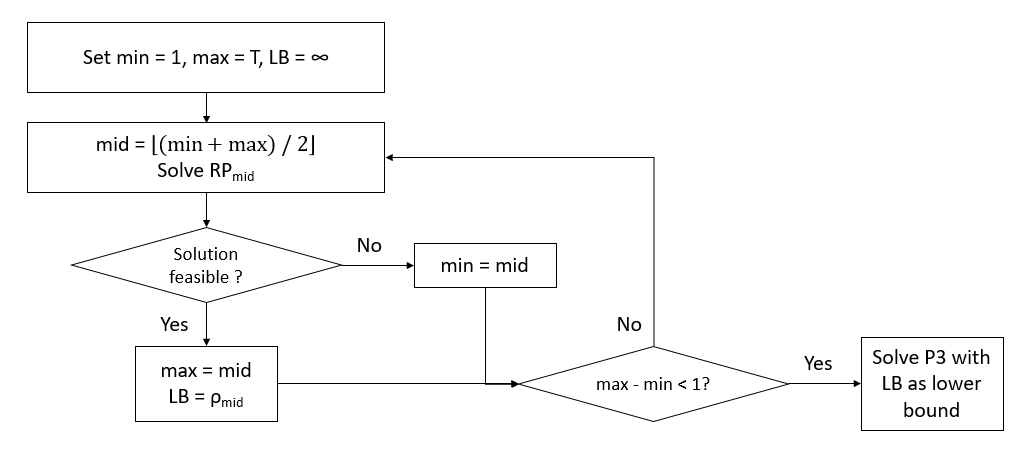
\includegraphics[width=\textwidth]{../imgs/BINARY.png}
		\caption{Flow chart of BINARY algorithm}
	\end{center}
\end{figure}
\noindent Applying a bisection search on the objective function of the linear relaxation comes to the same as applying a bisection search
on the objective function of the original problem. Indeed, an integer problem is infeasible if there is an infeasible relaxation of this problem.
Thus, the algorithm stops once the feasible solution with the lowest value of the objective has been found. \\\\
The main defect of this method is that it cannot be used alone, since it does not provide any upper bound.
Instead of combining BINARY with another technique for finding $UB$, we decided to implement one of the
double bound (DB) methods for the purpose of diversification among the algorithms discussed.
\section{Double bound algorithm}
Since comparing performance for different DB algorithms is not part
of the present project's objective, we only implemented one of them (that we did not assume to be the fastest
one). However, DB3 was reported in the paper to terminate in $\mathcal{O}(\log_3 T)$ iterations (against $\mathcal{O}(\log_2 T)$ iterations for DB1 and DB2).\\\\
Let:
\begin{itemize}
	\item $S$ be any nonempty subset of $T = \lbrace 1, ..., K \rbrace$
	\item $P(S)$ be the problem which is exactly the same as P3 except that all variables $z_k, k \in T\\S$ are dropped from P3
\end{itemize}\ \\
Calik and Tansel (2013) proposes and proves the following:\\\\
``Suppose $|S| > 2$. Let a and b be the smallest ad largest indices in S, respectively.\\
\begin{tabularx}{\textwidth}{l X}
(a) & If val($P(S)$) = $\rho_a$, then $r_p(F) \in \lbrace \rho_1, ..., \rho_a \rbrace$\\
(b) & If val($P(S)$) = $\rho_k$ for some $k$ with $a < k \leq b$, then $r_p(F) \in \lbrace \rho_{k'+1}, ..., \rho_k \rbrace$ where $k'$ is the largest index in $S$ which is smaller than $k$ \\
(c) & If val($P(S)$) = $\infty$, then $r_p(F) \in \lbrace \rho_{b+1}, ..., \rho_K \rbrace$''\\
\end{tabularx}\ \\\\
This proposition allows the construction of a more efficient search strategy based on the restriction of P3. 
Unfornately, the paper of Calik and Tansel (2013) made no mention of the feasibility of problem $P(S)$.
Indeed, with small values for both $\rho_a$ and $\rho_b$, $P(\{\rho_a, \rho_b\})$ may be infeasible.
This occurs when both $\rho_a$ and $\rho_b$ values are below the lowest objective value among feasible $RP_h$ solutions.
As a result, $P(S)$ may be infeasible for a certain set $S$ in exactly the same way that $RP_h$ may be infeasible for a certain index $h$.
For that reason, we set $min = b + 1$ if $P(S)$ is feasible, since both $a$ and $b$ would have led to an infeasible solution in BINARY algorithm.
In other words, all radius values less or equal to $\rho_b$ (> $\rho_a$) are discarded from the search space.
The double bound algorithm proposed by Calik and Tansel (2013) can now be schematized as follows:
\begin{figure}[H]
	\begin{center}
		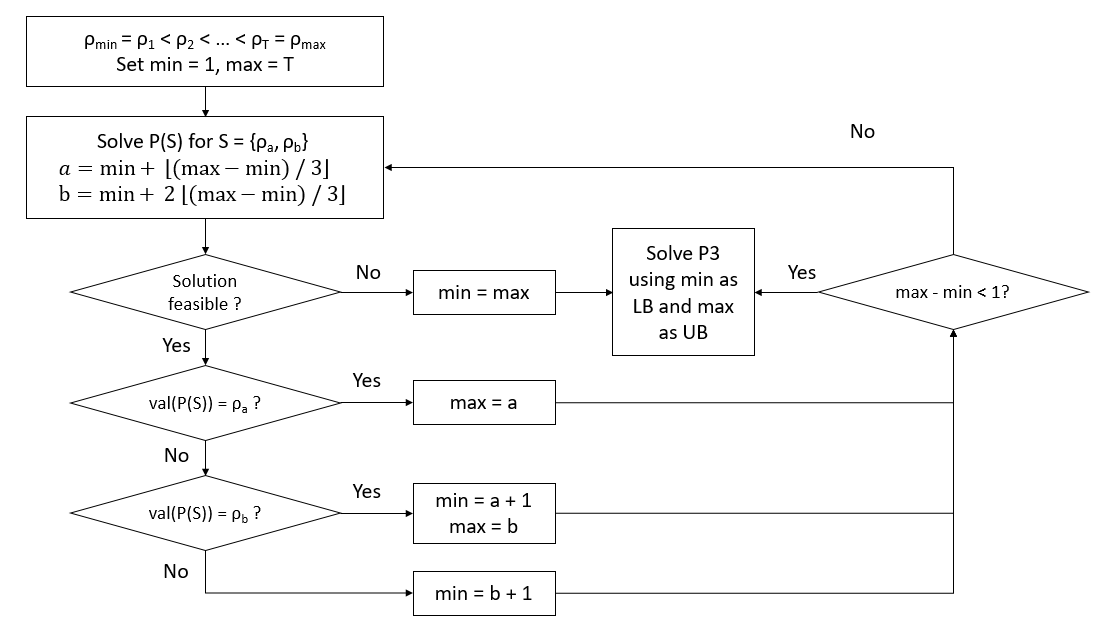
\includegraphics[width=\textwidth]{../imgs/DB3.png}
		\caption{Modified flow chart of DB3 algorithm}
	\end{center}
\end{figure}
\newpage
\chapter{Results}

These results were computed using the \verb+julia test_all.jl+ script which runs the two Cbc and GLPK solvers on all instances (30 easy instances and 10 hard instances) and writes the minimized objective function value and performance result of each instance in respective files in the \verb+results+ folder. For a better readability, we chose to make a separate result table per solver.

\section{Cbc}

\begin{table*}[h!]\centering
\ra{1.3}
\begin{tabular}{@{}rrrcrrcrr@{}}\toprule
& \multicolumn{2}{c}{P1} & \phantom{abc} & \multicolumn{2}{c}{P3 BIN} & \phantom{abc} & \multicolumn{2}{c}{P3 DB3}\\
\cmidrule{2-3} \cmidrule{5-6} \cmidrule{8-9}
& Obj & Time(s) & & Obj & Time(s) & & Obj & Time(s)\\ \midrule
instance10\_1\_1.dat & 75 & 2.422 & & 75 & 0.899 & & 75 & 0.214 \\
instance10\_1\_2.dat & 72 & 0.077 & & 72 & 0.018 & & 72 & 0.020 \\
instance10\_1\_3.dat & 85 & 0.080 & & 85 & 0.013 & & 85 & 0.018 \\
instance10\_1\_4.dat & 72 & 0.090 & & 72 & 0.014 & & 72 & 0.023 \\
instance10\_1\_5.dat & 70 & 0.089 & & 70 & 0.015 & & 70 & 0.020 \\
instance10\_2\_1.dat & 34 & 0.184 & & 34 & 0.019 & & 34 & 0.024 \\
instance10\_2\_2.dat & 43 & 0.123 & & 43 & 0.113 & & 43 & 0.050 \\
instance10\_2\_3.dat & 46 & 0.183 & & 46 & 0.039 & & 46 & 0.031 \\
instance10\_2\_4.dat & 42 & 0.103 & & 42 & 0.073 & & 42 & 0.032 \\
instance10\_2\_5.dat & 29 & 0.166 & & 29 & 0.040 & & 29 & 0.040 \\
instance10\_5\_1.dat & 9 & 0.132 & & 9 & 0.200 & & 9 & 0.015 \\
instance10\_5\_2.dat & 10 & 0.111 & & 10 & 0.100 & & 10 & 0.016 \\
instance10\_5\_3.dat & 9 & 0.100 & & 9 & 0.103 & & 9 & 0.030 \\
instance10\_5\_4.dat & 9 & 0.088 & & 9 & 0.132 & & 9 & 0.021 \\
instance10\_5\_5.dat & 11 & 0.097 & & 11 & 0.104 & & 11 & 0.015 \\
instance20\_2\_1.dat & 39 & 0.375 & & 39 & 0.293 & & 39 & 0.106 \\
instance20\_2\_2.dat & 53 & 1.570 & & 53 & 1.249 & & 53 & 0.136 \\
instance20\_2\_3.dat & 55 & 1.312 & & 55 & 0.365 & & 55 & 0.121 \\
instance20\_2\_4.dat & 51 & 1.163 & & 51 & 0.163 & & 51 & 0.166 \\
instance20\_2\_5.dat & 55 & 1.333 & & 55 & 0.920 & & 55 & 0.104 \\
instance20\_4\_1.dat & 21 & 0.260 & & 21 & 0.311 & & 21 & 0.043 \\
instance20\_4\_2.dat & 24 & 0.327 & & 24 & 0.061 & & 24 & 0.053 \\
instance20\_4\_3.dat & 23 & 0.261 & & 23 & 0.067 & & 23 & 0.088 \\
instance20\_4\_4.dat & 17 & 0.448 & & 17 & 0.074 & & 17 & 0.096 \\
instance20\_4\_5.dat & 22 & 0.342 & & 22 & 0.524 & & 22 & 0.080 \\
\end{tabular}
\end{table*}
\newpage
\begin{table*}[h!]\centering
\ra{1.3}
\begin{tabular}{@{}rrrcrrcrr@{}}\toprule
& \multicolumn{2}{c}{P1} & \phantom{abc} & \multicolumn{2}{c}{P3 BIN} & \phantom{abc} & \multicolumn{2}{c}{P3 DB3}\\
\cmidrule{2-3} \cmidrule{5-6} \cmidrule{8-9}
& Obj & Time(s) & & Obj & Time(s) & & Obj & Time(s)\\ \midrule
instance20\_10\_1.dat & 3 & 0.046 & & 3 & 0.863 & & 3 & 0.057 \\
instance20\_10\_2.dat & 4 & 0.152 & & 4 & 0.892 & & 4 & 0.026 \\
instance20\_10\_3.dat & 7 & 0.235 & & 7 & 0.874 & & 7 & 0.029 \\
instance20\_10\_4.dat & 4 & 0.136 & & 4 & 1.533 & & 4 & 0.033 \\
instance20\_10\_5.dat & 7 & 0.372 & & 7 & 1.616 & & 7 & 0.037 \\
instance1.dat & 127 & 140.100 & & 127 & 450.646 & & 127 & 3.105 \\
instance2.dat & 98 & 54.714 & & 98 & 12.602 & & 98 & 2.828 \\
instance3.dat & 93 & 71.143 & & 93 & 15.900 & & 93 & 1.524 \\
instance4.dat & 74 & 9.899 & & 74 & 19.966 & & 74 & 0.620 \\
instance5.dat & 48 & 6.591 & & 48 & 26.465 & & 48 & 0.923 \\
instance6.dat & 84 & 1109.202 & & 84 & 103.477 & & 84 & 2.178 \\
instance7.dat & 64 & 706.315 & & 64 & 40.686 & & 64 & 0.828 \\
instance8.dat & 55 & 572.170 & & 55 & 74.232 & & 55 & 3.316 \\
instance9.dat & 37 & 143.099 & & 37 & 63.442 & & 37 & 1.209 \\
instance10.dat & 20 & 32.296 & & 20 & 60.019 & & 20 & 0.821 \\
\bottomrule
\end{tabular}
\end{table*}\ \\

\begin{center}
\textbf{Average computation time}
\end{center}
\begin{table*}[h!]\centering
\ra{1.3}
\begin{tabular}{@{}rrcrcr@{}}\toprule
& \multicolumn{1}{c}{P1} & \phantom{abc} & \multicolumn{1}{c}{P3 BIN} & \phantom{abc} & \multicolumn{1}{c}{P3 DB3}\\
& Time(s) & & Time(s) & & Time(s)\\ \midrule
easy instances & 0.413 & & 0.389 & & 0.058 \\
hard instances & 284.553 & & 86.743 & & 1.735 \\
\bottomrule
\end{tabular}
\end{table*}\ \\

\newpage
\section{GLPK}

\begin{table*}[h!]\centering
\ra{1.3}
\begin{tabular}{@{}rrrcrrcrr@{}}\toprule
& \multicolumn{2}{c}{P1} & \phantom{abc} & \multicolumn{2}{c}{P3 BIN} & \phantom{abc} & \multicolumn{2}{c}{P3 DB3}\\
\cmidrule{2-3} \cmidrule{5-6} \cmidrule{8-9}
& Obj & Time(s) & & Obj & Time(s) & & Obj & Time(s)\\ \midrule
instance10\_1\_1.dat & 75 & 3.143 & & 75 & 0.917 & & 75 & 0.206 \\
instance10\_1\_2.dat & 72 & 0.026 & & 72 & 0.002 & & 72 & 0.003 \\
instance10\_1\_3.dat & 85 & 0.024 & & 85 & 0.004 & & 85 & 0.002 \\
instance10\_1\_4.dat & 72 & 0.017 & & 72 & 0.003 & & 72 & 0.004 \\
instance10\_1\_5.dat & 70 & 0.027 & & 70 & 0.005 & & 70 & 0.005 \\
instance10\_2\_1.dat & 34 & 0.043 & & 34 & 0.006 & & 34 & 0.003 \\
instance10\_2\_2.dat & 43 & 0.042 & & 43 & 0.059 & & 43 & 0.003 \\
instance10\_2\_3.dat & 46 & 0.037 & & 46 & 0.004 & & 46 & 0.003 \\
instance10\_2\_4.dat & 42 & 0.035 & & 42 & 0.012 & & 42 & 0.003 \\
instance10\_2\_5.dat & 29 & 0.036 & & 29 & 0.005 & & 29 & 0.008 \\
instance10\_5\_1.dat & 9 & 0.008 & & 9 & 0.006 & & 9 & 0.003 \\
instance10\_5\_2.dat & 10 & 0.021 & & 10 & 0.007 & & 10 & 0.003 \\
instance10\_5\_3.dat & 9 & 0.030 & & 9 & 0.007 & & 9 & 0.003 \\
instance10\_5\_4.dat & 9 & 0.019 & & 9 & 0.005 & & 9 & 0.004 \\
instance10\_5\_5.dat & 11 & 0.015 & & 11 & 0.006 & & 11 & 0.003 \\
instance20\_2\_1.dat & 39 & 0.864 & & 39 & 0.018 & & 39 & 0.012 \\
instance20\_2\_2.dat & 53 & 1.000 & & 53 & 0.122 & & 53 & 0.013 \\
instance20\_2\_3.dat & 55 & 1.252 & & 55 & 0.057 & & 55 & 0.013 \\
instance20\_2\_4.dat & 51 & 1.227 & & 51 & 0.064 & & 51 & 0.009 \\
instance20\_2\_5.dat & 55 & 1.113 & & 55 & 0.120 & & 55 & 0.012 \\
instance20\_4\_1.dat & 21 & 0.093 & & 21 & 0.024 & & 21 & 0.011 \\
instance20\_4\_2.dat & 24 & 2.430 & & 24 & 0.012 & & 24 & 0.007 \\
instance20\_4\_3.dat & 23 & 0.841 & & 23 & 0.020 & & 23 & 0.009 \\
instance20\_4\_4.dat & 17 & 1.529 & & 17 & 0.031 & & 17 & 0.009 \\
instance20\_4\_5.dat & 22 & 0.427 & & 22 & 0.088 & & 22 & 0.011 \\
instance20\_10\_1.dat & 3 & 0.546 & & 3 & 0.027 & & 3 & 0.007 \\
instance20\_10\_2.dat & 4 & 0.148 & & 4 & 0.030 & & 4 & 0.005 \\
instance20\_10\_3.dat & 7 & 0.346 & & 7 & 0.024 & & 7 & 0.012 \\
instance20\_10\_4.dat & 4 & 0.320 & & 4 & 0.031 & & 4 & 0.007 \\
instance20\_10\_5.dat & 7 & 0.219 & & 7 & 0.023 & & 7 & 0.012 \\
\end{tabular}
\end{table*}
\newpage
\begin{center}
\textbf{Average computation time}
\end{center}
\begin{table*}[h!]\centering
\ra{1.3}
\begin{tabular}{@{}rrcrcr@{}}\toprule
& \multicolumn{1}{c}{P1} & \phantom{abc} & \multicolumn{1}{c}{P3 BIN} & \phantom{abc} & \multicolumn{1}{c}{P3 DB3}\\
& Time(s) & & Time(s) & & Time(s)\\ \midrule
easy instances & 0.529 & & 0.058 & & 0.013 \\
\bottomrule
\end{tabular}
\end{table*}\ \\\\
\textbf{Important note:} unlike with Cbc, P1 forumulations of hard instances couldn't be solved in a reasonable time using GLPK
\newpage
\chapter{Discussion}
Regarding the results computed hereabove, we can observe that P1, P3 BINARY and P3 DB3 algorithms all reached the same (optimum) value for all instances. On the other hand, the computation time to reach an optimum solution varies significantly between the different algorithms, especially on the hard instances where P1, P3 BINARY and P3 DB3 report an average computation time (in seconds) of 284.553, 86.743 and 1.735 respectively. P3 DB3's performances seems to scale very well with the instances complexity.\\\\
Regarding the details of the solutions reached by the P1, P3 BINARY and P3 DB3 algorithms, we can observe different behaviors depending on the solver used to solve the instance:
\begin{itemize}
	\item Cbc: the locations of the selected \textit{p} centers are identical for the easy instances but different for the hard instances depending on the algorithm used to compute the solution.
	\item GLPK: the locations of the selected \textit{p} centers are different for some of the easy instances depending on the algorithm used to compute the solution. Unfortunately, the behavior of GLPK on hard instances couldn't be verified because GLPK couldn't solve these instances in a reasonable time.
\end{itemize}\ \\
To better illustrate the application of the BINARY and DB3 algorithms' diagrams on concrete instances, these two graphs hereunder plot respectively the search space for finding the low bound (BINARY) and the evolution of lower and upper bounds (DB3) when executing the algorithms on different instances.
\begin{figure}[h!]
    \begin{center}
        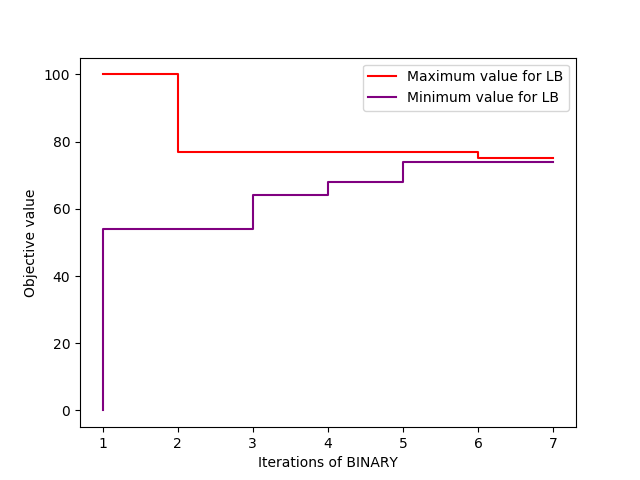
\includegraphics[width=0.72\textwidth]{../imgs/binary_bounds.png}
        \caption{Search space of BINARY algorithm for finding the
        lower bound \\ on easy/instance10\_1\_1.dat}
    \end{center}
\end{figure}
\newpage
\begin{figure}[h!]
    \begin{center}
        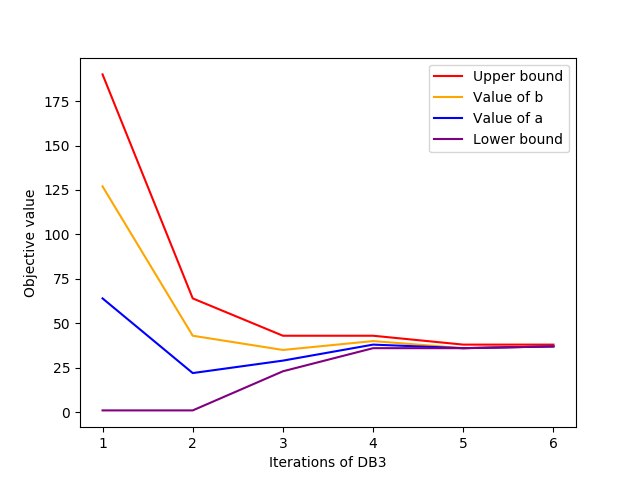
\includegraphics[width=0.72\textwidth]{../imgs/db3_bounds.png}
        \caption{Evolution of lower and upper bounds using DB3 \\
        algorithm on instance hard/instance9.dat}
    \end{center}
\end{figure}


%\chapter*{Annexes}
%\includepdf[pages={-}]{code/xemins.pdf}
%\includepdf[pages={-}]{code/main.pdf}

\end{document}
